\PassOptionsToPackage{unicode=true}{hyperref} % options for packages loaded elsewhere
\PassOptionsToPackage{hyphens}{url}
\documentclass[11pt,dvipsnames,ignorenonframetext,aspectratio=169]{beamer}
\IfFileExists{pgfpages.sty}{\usepackage{pgfpages}}{}
\setbeamertemplate{caption}[numbered]
\setbeamertemplate{caption label separator}{: }
\setbeamercolor{caption name}{fg=normal text.fg}
\beamertemplatenavigationsymbolsempty
\usepackage{lmodern}
\usepackage{amssymb,amsmath}
\usepackage{ifxetex,ifluatex}
\usepackage{fixltx2e} % provides \textsubscript
\ifnum 0\ifxetex 1\fi\ifluatex 1\fi=0 % if pdftex
  \usepackage[T1]{fontenc}
  \usepackage[utf8]{inputenc}
\else % if luatex or xelatex
  \ifxetex
    \usepackage{mathspec}
  \else
    \usepackage{fontspec}
\fi
\defaultfontfeatures{Ligatures=TeX,Scale=MatchLowercase}







\fi

  \usetheme[]{monash}

  \usecolortheme{monashwhite}


% A default size of 24 is set in beamerthememonash.sty

% Title page
\setbeamertemplate{title page}
{\placefig{-0.01}{-0.01}{width=1.01\paperwidth,height=1.01\paperheight}{falcon.png}
\begin{textblock}{7.5}(1,2.8)\usebeamerfont{title}
{\color{white}\raggedright\par\inserttitle}
\end{textblock}
\begin{textblock}{7.5}(1,7)
{\color{white}\raggedright{\insertauthor}\mbox{}\\[0.2cm]
\insertdate}
\end{textblock}}


  \useinnertheme{rounded}

  \useoutertheme{smoothtree}

% use upquote if available, for straight quotes in verbatim environments
\IfFileExists{upquote.sty}{\usepackage{upquote}}{}
% use microtype if available
\IfFileExists{microtype.sty}{%
  \usepackage{microtype}
  \UseMicrotypeSet[protrusion]{basicmath} % disable protrusion for tt fonts
}{}


\newif\ifbibliography
  \usepackage[round]{natbib}
  \bibliographystyle{plainnat}


\hypersetup{
      pdftitle={Precision agriculture},
            colorlinks=true,
    linkcolor=red,
    citecolor=Blue,
    urlcolor=lightgrayd,
    breaklinks=true}
%\urlstyle{same}  % Use monospace font for urls







% Prevent slide breaks in the middle of a paragraph:
\widowpenalties 1 10000
\raggedbottom

  \AtBeginPart{
    \let\insertpartnumber\relax
    \let\partname\relax
    \frame{\partpage}
  }
  \AtBeginSection{
    \ifbibliography
    \else
      \let\insertsectionnumber\relax
      \let\sectionname\relax
      \frame{\sectionpage}
    \fi
  }
  \AtBeginSubsection{
    \let\insertsubsectionnumber\relax
    \let\subsectionname\relax
    \frame{\subsectionpage}
  }



\setlength{\parindent}{0pt}
\setlength{\parskip}{6pt plus 2pt minus 1pt}
\setlength{\emergencystretch}{3em}  % prevent overfull lines
\providecommand{\tightlist}{%
  \setlength{\itemsep}{0pt}\setlength{\parskip}{0pt}}

  \setcounter{secnumdepth}{0}


%% Monash overrides
\AtBeginSection[]{
   \frame<beamer>{
   \frametitle{Outline}\vspace*{0.2cm}
   
   \tableofcontents[currentsection,hideallsubsections]
  }}

% Redefine shaded environment if it exists (to ensure text is black)
\ifcsname Shaded\endcsname
  \definecolor{shadecolor}{RGB}{225,225,225}
  \renewenvironment{Shaded}{\color{black}\begin{snugshade}\color{black}}{\end{snugshade}}
\fi
%%


  \usepackage{setspace}
  \usepackage{wasysym}
  % \usepackage{footnote} % don't use this this breaks all
  \usepackage{fontenc}
  \usepackage{fontawesome}
  \usepackage{booktabs,siunitx}
  \usepackage{longtable}
  \usepackage{array}
  \usepackage{multirow}
  \usepackage{wrapfig}
  \usepackage{float}
  \usepackage{colortbl}
  \usepackage{pdflscape}
  \usepackage{tabu}
  \usepackage{threeparttable}
  \usepackage{threeparttablex}
  \usepackage[normalem]{ulem}
  \usepackage{makecell}
  \usepackage{xcolor}
  \usepackage{tikz} % required for image opacity change
  \usepackage[absolute,overlay]{textpos} % for text formatting
  \usepackage{chemfig}
  \usepackage[skip=0.333\baselineskip]{caption}
  % \newcommand*{\AlignChar}[1]{\makebox[1ex][c]{\ensuremath{\scriptstyle#1}}}%

  % this font option is amenable for beamer
  \setbeamerfont{caption}{size=\tiny}
  \singlespacing
  \definecolor{lightgrayd}{gray}{0.95}
  \definecolor{skyblued}{rgb}{0.65, 0.6, 0.94}
  \definecolor{oranged}{RGB}{245, 145, 200}

  % \newlength{\cslhangindent}
  % \setlength{\cslhangindent}{1.5em}
  % \newenvironment{cslreferences}%
  %   {\setlength{\parindent}{0pt}%
  %   \everypar{\setlength{\hangindent}{\cslhangindent}}\ignorespaces}%
  %   {\par}


  \newcommand{\bcolumns}{\begin{columns}[T, onlytextwidth]}
  \newcommand{\ecolumns}{\end{columns}}

  \newcommand{\bdescription}{\begin{description}}
  \newcommand{\edescription}{\end{description}}

  \newcommand{\bitemize}{\begin{itemize}}
  \newcommand{\eitemize}{\end{itemize}}
  \AtBeginSubsection{}

  \title[]{Precision agriculture}

  \subtitle{Concepts and techniques, tools of precison agriculture used
in abroad and Nepal; STCR approach}

  \author[
        Deependra Dhakal\\
Assistant Professor\\
\textit{ddhakal.rookie@gmail.com}\\
\url{https://rookie.rbind.io}
    ]{Deependra Dhakal\\
Assistant Professor\\
\textit{ddhakal.rookie@gmail.com}\\
\url{https://rookie.rbind.io}}


\date[
      
  ]{
    }

\begin{document}

% Hide progress bar and footline on titlepage
  \begin{frame}[plain]
  \titlepage
  \end{frame}


   \frame<beamer>{
   \frametitle{Outline}\vspace*{0.2cm}
   
   \tableofcontents[hideallsubsections]
  }

\hypertarget{concepts-and-techniques}{%
\section{Concepts and techniques}\label{concepts-and-techniques}}

\begin{frame}{}
\protect\hypertarget{section}{}
\begin{alert}{Course objectives:}
The objective of this course is to provide theory as well as hands-on skill to students for various applications in Remote-sensing (RS), GIS and related technology for precision agriculture.
\end{alert}

\textit{"It would be a simple matter to describe the earth's surface if it were the same everywhere. The environment, however, is not like that: there is almost endless variety."}

\raggedleft --- Webster and Oliver (1990)
\end{frame}

\begin{frame}{Meaning and definition}
\protect\hypertarget{meaning-and-definition}{}
\begin{itemize}
\tightlist
\item
  Management of \alert{variability} in the dimensions of both space and
  time!
\item
  Any component of production agriculture -- plant genetic resource,
  production inputs, farm machinery, and farm operators -- are variable.
\item
  All of these can be included in the realm of precision agriculture,
  not only the soil.
\item
  Aspects include:

  \begin{itemize}
  \footnotesize
  \item Variability of soil resource base
  \item Weather
  \item Plant genetics
  \item Crop diversity
  \item Machinery performance
  \item Most physical, chemical and biological inputs used in the crop production (synthetic/natural)
  \end{itemize}
\item
  By necessity, all are framed within the context of the variable
  socio-economic aspects of production agriculture.

  \begin{itemize}
  \footnotesize
  \item to be successful on the farm, precision agriculture must fit the needs and capabilities of the farmer and must be profitable.
  \end{itemize}
\end{itemize}
\end{frame}

\begin{frame}{}
\protect\hypertarget{section-1}{}
\begin{columns}[T, onlytextwidth]
\column{0.6\textwidth}
\begin{itemize}
\small
\item Managing soil and crops in space and time is the sustainable management principle for the 21st century, exemplified by:
  \begin{itemize}
  \footnotesize
  \item Farming by soilscapes
  \item Managing zones within the field
  \item Managing the non-crop period
  \end{itemize}
\item Concerns of the technology:
  \begin{itemize}
  \footnotesize
  \item assistive technologies enabling the efficient use
  \item agronomic feasibility
  \item environmental efficacy
  \item performance with respect to economic and social impacts
  \end{itemize}
\end{itemize}

\column{0.4\textwidth}

\begin{figure}

{\centering 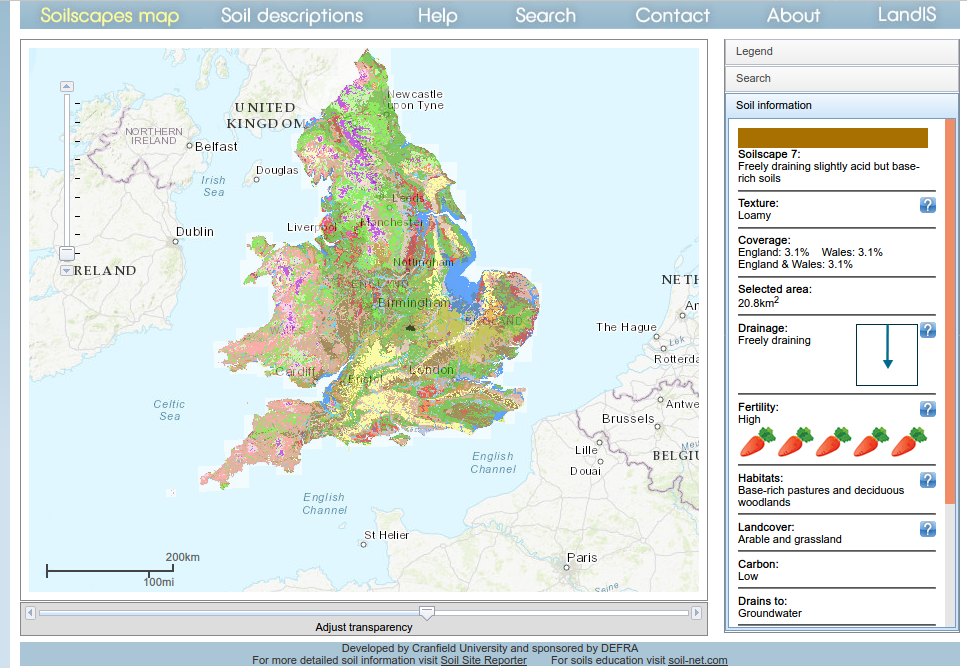
\includegraphics[width=0.98\linewidth]{../images/soilscape_uk_2022-09-14 17-57-00} 

}

\caption{Georefrenced soilscapes map of UK. Source: \url{http://www.landis.org.uk/soilscapes/}}\label{fig:soilscape-uk}
\end{figure}
\end{columns}

\begin{block}{Known names of Precision agriculture}
Farming by the foot, farming by soil, variable rate technology (VRT), spatially variable farming, prescription farming, site-specific crop production, site-specific management...
\end{block}
\end{frame}

\begin{frame}{}
\protect\hypertarget{section-2}{}
\begin{block}{Stafford (1996)}
"The targeting of inputs to arable crop production according to crop requirements on a localized basis"
\end{block}

\begin{itemize}
\tightlist
\item
  4R principle:

  \begin{itemize}
  \tightlist
  \item
    Right thing
  \item
    Right place
  \item
    Right time
  \item
    Right way
  \end{itemize}
\end{itemize}

\begin{block}{NRC, Board on Agriculture Committee, US}
"A management strategy that uses information technologies to bring data from multiple sources to bear on decisions associated with crop production."
\end{block}

``Precision agriculture is the application of technologies and
principles to manage spatial and temporal variability associated with
all aspects of agricultural production for the purpose of improving crop
performance and environmental quality.''
\end{frame}

\begin{frame}{Precision versus Accuracy}
\protect\hypertarget{precision-versus-accuracy}{}
\begin{figure}
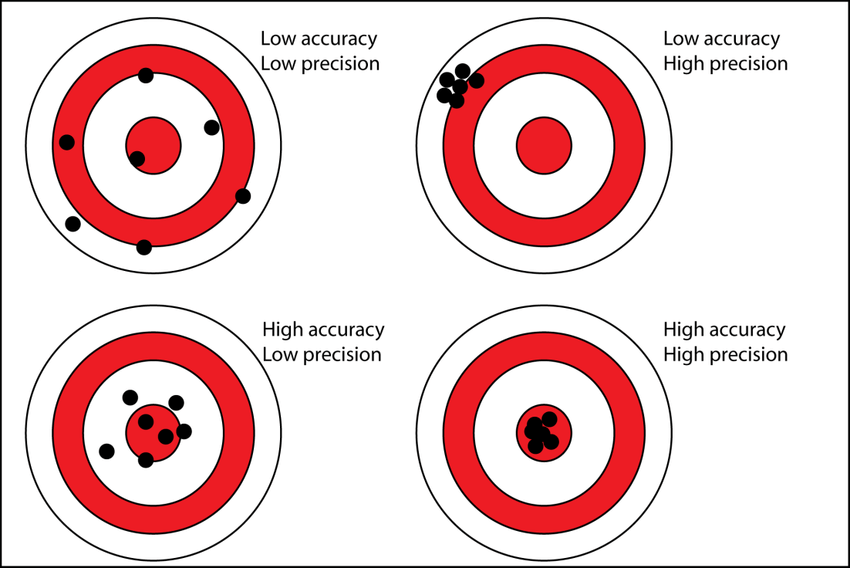
\includegraphics[width=0.36\linewidth]{../images/precision_vs_accuracy_bulls_eye_view} \caption{Precision verus accuracy. Something can be precise but not accurate.}\label{fig:precision-vs-accuracy}
\end{figure}

\footnotesize

\begin{itemize}
\tightlist
\item
  Nature of computers makes it easy to imply more \emph{precision} than
  was possible in various aspects of data collection, analysis,
  computation in precision agriculture.
\item
  Precision refers to the limits on the measurement scale between which
  the true measurement is believed to lie, implied by the number of
  digits reported for a measurement.

  \begin{itemize}
  \tightlist
  \item
    A pH of 5.4 or 5.44
  \end{itemize}
\end{itemize}
\end{frame}

\begin{frame}{The idea}
\protect\hypertarget{the-idea}{}
\begin{itemize}
\tightlist
\item
  Intuitively appealing

  \begin{itemize}
  \tightlist
  \item
    scientific principles of management of soils, crops, and pests
  \item
    arguing against a management philosophy that aims at matching inputs
    to the exact needs everywhere is not easy.
  \end{itemize}
\item
  Successful implementation of precision agriculture depends on numerous
  factors, including:

  \begin{itemize}
  \tightlist
  \item
    the extent to which conditions within a field are known and
    manageable,
  \item
    the adequacy of input recommendations,
  \item
    the degree of application control,
  \item
    the degree of support through private and public infrastructures,
  \item
    the expectations of individual (how do you know maximum potential
    has been reached?)
  \end{itemize}
\end{itemize}
\end{frame}

\begin{frame}{Basic components}
\protect\hypertarget{basic-components}{}
\begin{itemize}
\tightlist
\item
  Measurement and understanding of variability
\item
  Use information to manage this variability by matching inputs to
  conditions within fields using
  \alert{site-specific management recommendation}
\item
  Mechanism to control the accuracy of site-specific inputs
\item
  Provide for the measurement and recording of the efficiency and
  efficacy of these site-specific practices in order to assess value on
  and off the farm.
\end{itemize}
\end{frame}

\begin{frame}{Precision fertilizer management: An example use case}
\protect\hypertarget{precision-fertilizer-management-an-example-use-case}{}
\begin{itemize}
\tightlist
\item
  In conventional farming system, blanket application of high amounts of
  nitrogen fertilizer has been in practice.
\item
  Soil's nutrient mobility potential (due to soil physical and chemical
  properties), soil moisture, crop/variety specific demand and field
  micro-variations are unaccounted.

  \begin{itemize}
  \tightlist
  \item
    N losess are due to \(NO^{-}_3\) leaching and \(NH^{+}_4\)
    volatilization
  \item
    Higer cost of production (added cost of input fertilizer purchase in
    order to compensate for loss)
  \end{itemize}
\item
  Collecting in-season biomass sample for analysis is cost prohibitive,
  labor intensive and destructive.
\end{itemize}
\end{frame}

\begin{frame}{Enabling technologies}
\protect\hypertarget{enabling-technologies}{}
\begin{enumerate}
\tightlist
\item
  Computers
\item
  Global positioning system (GPS)
\item
  Geographic information system (GIS)
\item
  Sensors
\item
  Application control
\end{enumerate}
\end{frame}

\begin{frame}{Early history}
\protect\hypertarget{early-history}{}
\begin{columns}[T, onlytextwidth]

\column{0.75\textwidth}

\begin{itemize}
\small
\item Pierre Robert is often regarded as the father of precision farming
\item In 1982, Robert defended his PhD dissertation titled "Evaluation of some remote sensing techniques for soil and crop management"
  \begin{itemize}
  \footnotesize
  \item Showed that color infrared (CIR) aerial photography could be used to detect "Problems relating to drainage, erosion, germination, grass and weed control, crop stand damage and machinery malfunction."
  \item Suggested that CIR data could be used to build a "farm information and management system containing precisely located natural and cultural data to improve cost efficiency of future cultural practices. Such improvement could come, for example, from adjusting seed density, herbicide control or fertilization in response to detected field problems"
  \end{itemize}
\item Notes that anomalous reflectance patterns from row-cropped fields were associated with soil series boundaries
\end{itemize}

\column{0.25\textwidth}

\begin{figure}
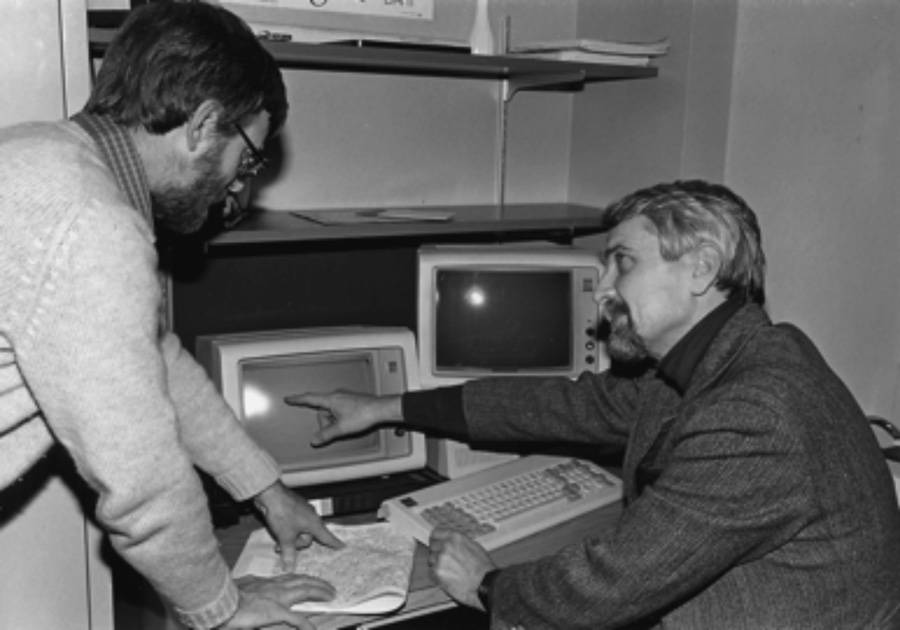
\includegraphics[width=0.99\linewidth]{../images/pierre-robert-in-development} \caption{Pierre Robert explaining his computerized farming by soil map database (circa 1985) to Jim Anderson at the University of Minnesota.}\label{fig:pierre-robers-computerized-farming}
\end{figure}

\end{columns}
\end{frame}

\hypertarget{tools-of-precision-agriculture}{%
\section{Tools of precision
agriculture}\label{tools-of-precision-agriculture}}

\begin{frame}{}
\protect\hypertarget{section-3}{}
\begin{itemize}
\tightlist
\item
  Soil sampling
\item
  Geostatistics and GIS
\item
  Farming by soil
\item
  Variable rate fertilizer
\item
  Site specific farming and management zones
\item
  GPS
\item
  Automated tractor navigation and robots
\item
  Yield mapping
\item
  Variable rate herbicide application
\item
  Variable rate irrigation
\item
  Remote sensing
\item
  Proximal sensing of soil and crops
\end{itemize}
\end{frame}

\begin{frame}{Precision agriculture in Nepal}
\protect\hypertarget{precision-agriculture-in-nepal}{}
\begin{itemize}
\tightlist
\item
  Attempt to land categorization using digital soil map
\item
  Micropropagation nurseries
\item
  Drip irrigation system
\item
  Use of cropping systems model of decision making
\item
  Use of laser land leveler
\item
  Rice planter
\item
  Drone sprayer
\end{itemize}
\end{frame}

\begin{frame}{}
\protect\hypertarget{section-4}{}
\begin{columns}[T, onlytextwidth]
\column{0.5\textwidth}

\begin{figure}
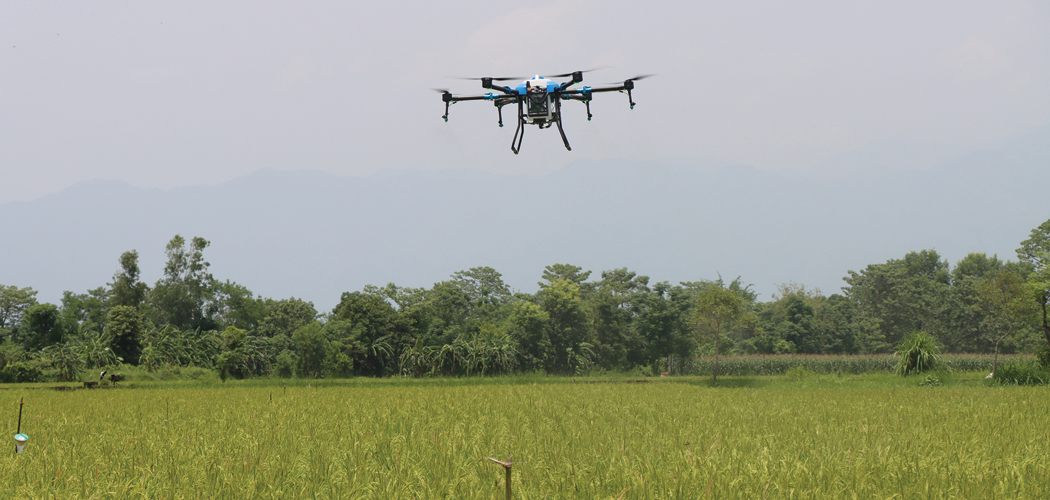
\includegraphics[width=0.98\linewidth]{../images/drone_pesticide_application} \caption{PMAMP, Chitwan using drones in the rice field for pesticide spray. The introduced drone of given design cost around NRS 1,500,000. It sprays the pesticide or liquid fertilizer 20 times as efficiently (requires lesser spray volume) as traditional hand held sprayer.}\label{fig:drone-spraying-pesticides-pmamp}
\end{figure}

\column{0.5\textwidth}

\begin{figure}
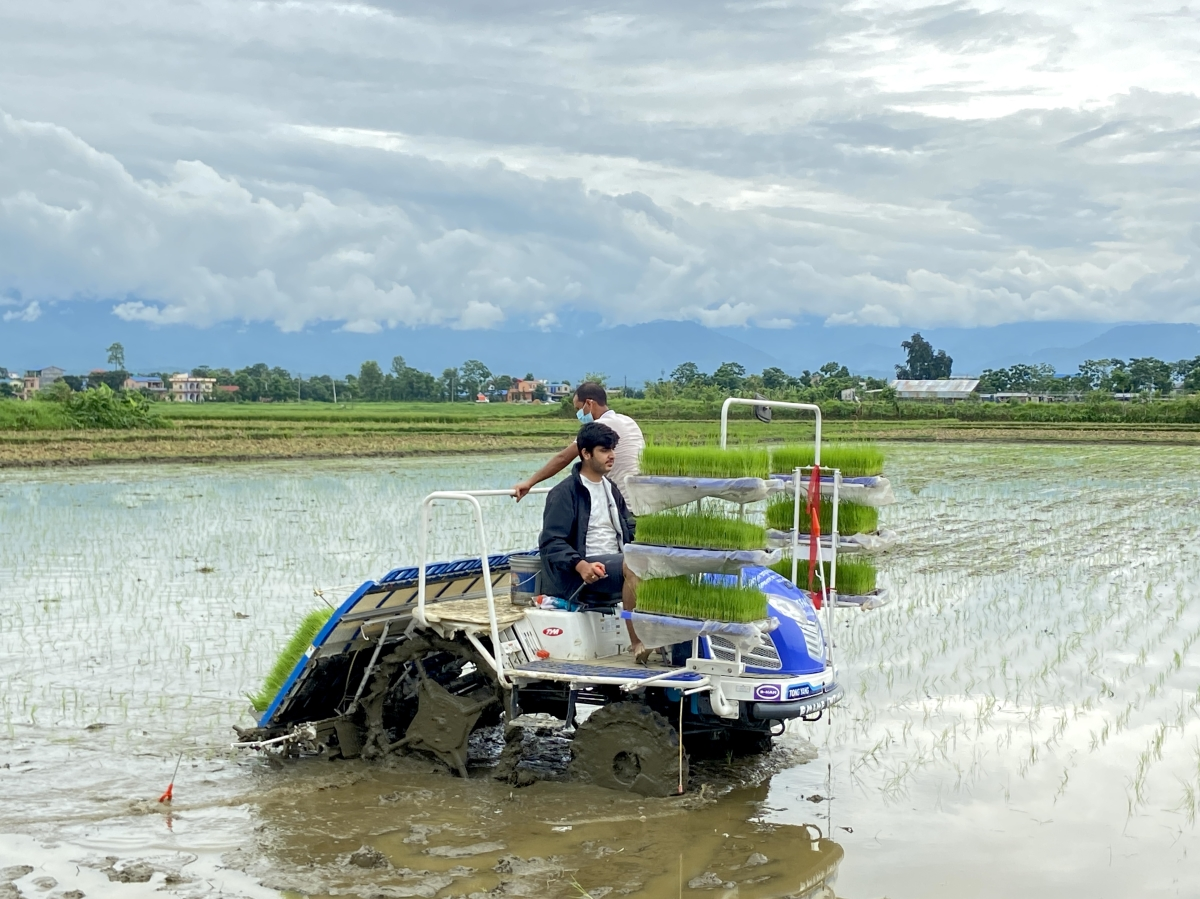
\includegraphics[width=0.98\linewidth]{../images/Mechanical-Transplanter-chitwan} \caption{An agriculture engineer operating rice transplanter. The PMAMP, Chitwan is trialing with mechanical aids to paddy plantation, management and harvest. The instruments are a four-wheel-drive riding-type rice planter, a combined harvester and plastic trays. A rice planter machine shown allows farmers to sow six saplings at a time instead of one and decreases the labour by 40-50 percent. The saplings are treated and kept in a tray that then efficiently places them into the soil. The machine can cover one bigha (around 72,900 square feet) of land per hour.}\label{fig:mechanical-rice-planter}
\end{figure}

\end{columns}
\end{frame}

\begin{frame}{}
\protect\hypertarget{section-5}{}
\begin{columns}[T,onlytextwidth]
\column{0.5\textwidth}

\begin{figure}
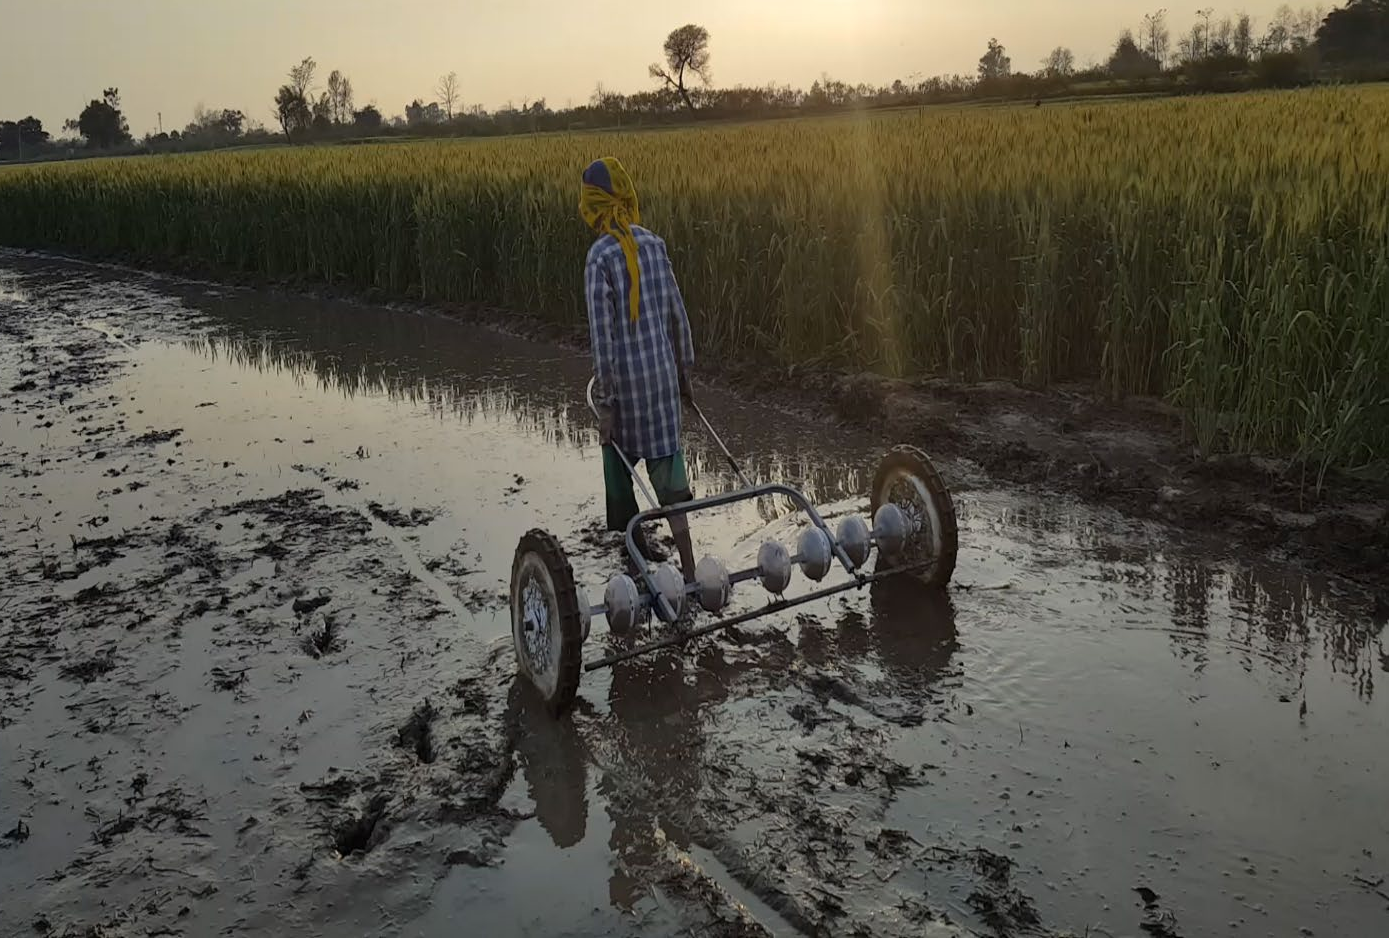
\includegraphics[width=0.7\linewidth]{../images/drum_seeder} \caption{Use of drum seeder in rice seeding (useful for DST). It has three drums for applying seeds and two hoppers for applying Granulated Urea, which were placed over a shaft.}\label{fig:drum-seeder}
\end{figure}


\begin{center}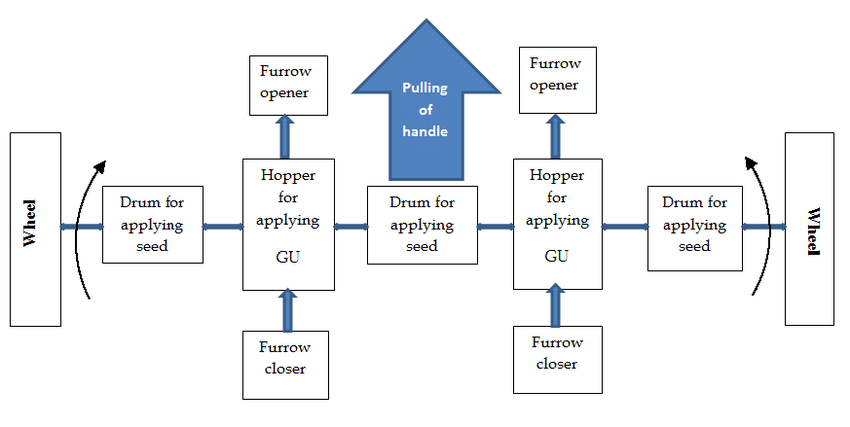
\includegraphics[width=0.6\linewidth]{../images/drum_seeder_mechanism} \end{center}

\column{0.5\textwidth}

\begin{figure}
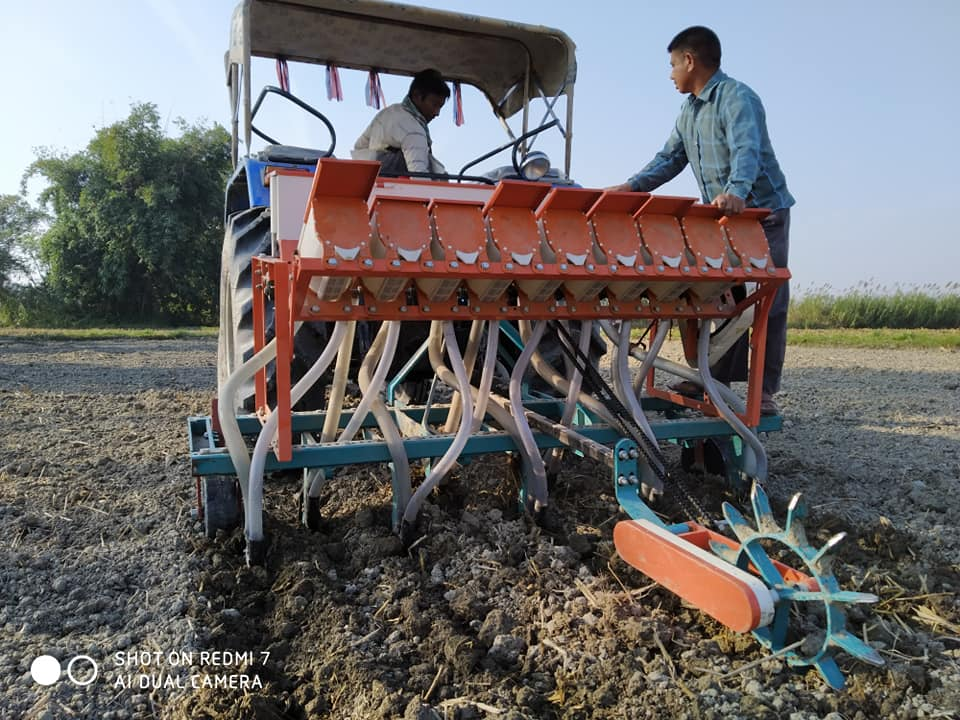
\includegraphics[width=0.9\linewidth]{../images/seed_cum_ferti_tilll_drill} \caption{Seed cum ferti till drill}\label{fig:seed-cum-ferti-till-drill}
\end{figure}

\end{columns}
\end{frame}

\begin{frame}{}
\protect\hypertarget{section-6}{}
\begin{figure}
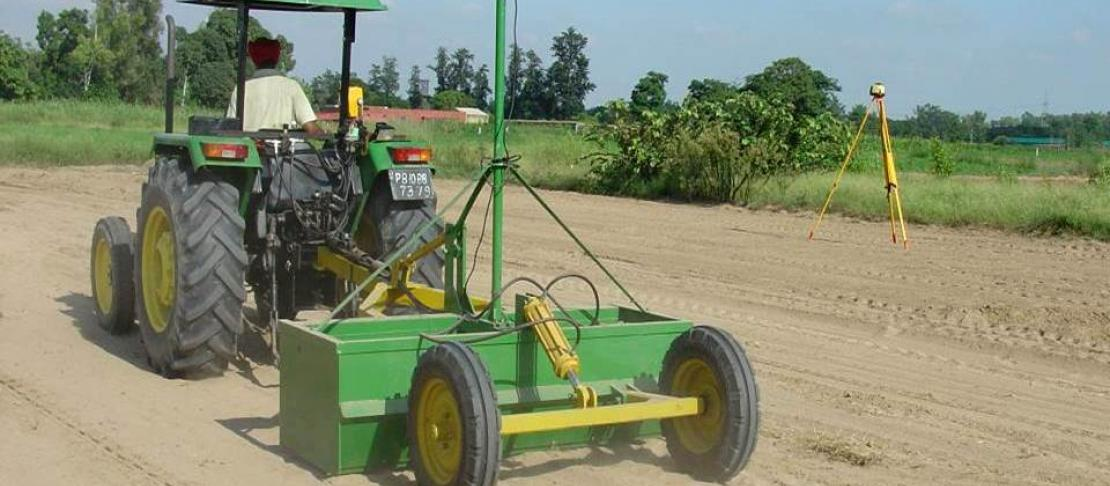
\includegraphics[width=0.45\linewidth]{../images/Laser_land_leveller} \caption{Laser guided drag bucket for land levelling. This ensures a flat table-top like land surface which increases water use efficiency as irrigated water reaches every part of the field with minimal run-off or water-logging. It reduces irrigation times in rice by 47-69 hours/hectare per season and in wheat by 10-12 hours/hectare per season. Increases yield by about 8 percent.}\label{fig:laser-land-leveler}
\end{figure}
\end{frame}

\begin{frame}{Specific use cases in PA}
\protect\hypertarget{specific-use-cases-in-pa}{}
\begin{itemize}
\tightlist
\item
  Soil water monitoring/ Inefficient or broken drainage
\item
  Seed germination, plant density and crop growth rate,
\item
  Viral, microbial, fungal diseases and insects' pests diagnostics,
\item
  Weeds and other unwanted plant species monitoring,
\item
  Plant nutrient deficiency diagnostics and management,
\item
  Soil health and Soil-Microbes analysis,
\item
  Food nutrients composition and Phyto-chemicals analysis,
\item
  Weather forecast for cultivation
\item
  Calendar for agricultural crop cultivation
\end{itemize}
\end{frame}

\begin{frame}{Limitations}
\protect\hypertarget{limitations}{}
\begin{itemize}
\tightlist
\item
  Land come with fixed size
\item
  Despite all of these state of precision agriculture from a systems
  perspective is analogous to the early days of no-tillage crop
  production.
\item
  No perfect form of precision agricultural systems exist as of yet!
\item
  Only components of traditional crop management systems have been
  addressed separately regarding their potential for site-specific
  management, most notably soil fertility.
\item
  Management parameters that vary spatially, those with high temporal
  correlations (e.g., liming) will be more easily managed with precision
  agriculture than those with large temporal variance (e.g., mobile
  insects).
\end{itemize}
\end{frame}

\hypertarget{stcr-approach-for-precision-agriculture}{%
\section{STCR approach for precision
agriculture}\label{stcr-approach-for-precision-agriculture}}

\begin{frame}{Soil test crop response (STCR)}
\protect\hypertarget{soil-test-crop-response-stcr}{}
\bcolumns
\column{0.45\textwidth}
\footnotesize

\begin{itemize}
\tightlist
\item
  STCR is technique based on soil testing which aims to make
  quantitative fertilizer recommendation for the profit maximizing dose
  of fertilizer in the given parcel of land for a specific crop.
\item
  Testing generally involves analysis of chemical constitution as well
  as physical attributes of the soil with standardized protocols.
  Primarily, STCR study aim to:

  \begin{itemize}
  \footnotesize
  \item Study the relationship between soil test values for available N, P, K and yield response to important crops.
  \item Derive yield equations as function of fertilizer compositions for crops to make site specific recommendation.
  \end{itemize}
\end{itemize}

\column{0.55\textwidth}

\begin{figure}
  \begin{columns}[T,onlytextwidth]
  \column{.7\linewidth}
  \begin{center}
  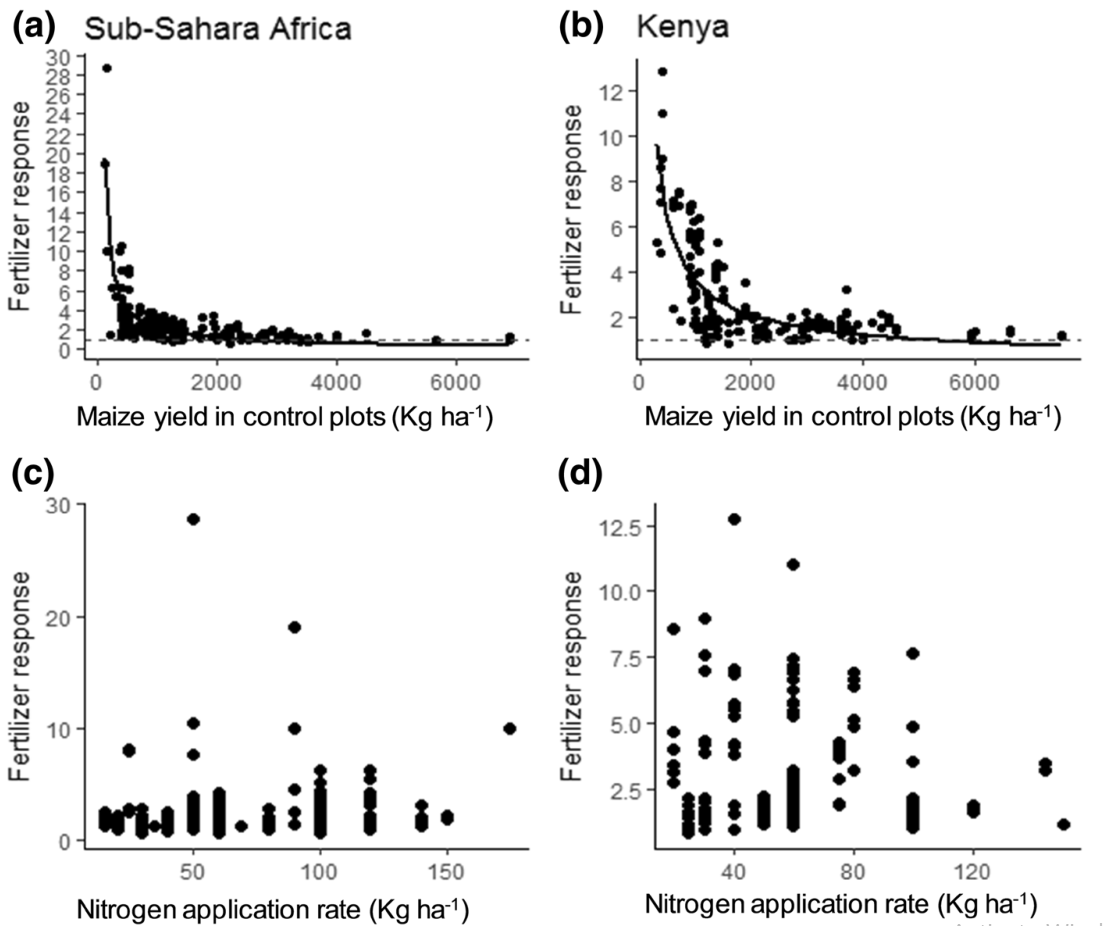
\includegraphics[width=0.85\linewidth]{../images/fertilizer_response_sub_saharan_africa.PNG}
  \end{center}
  \begin{center}
  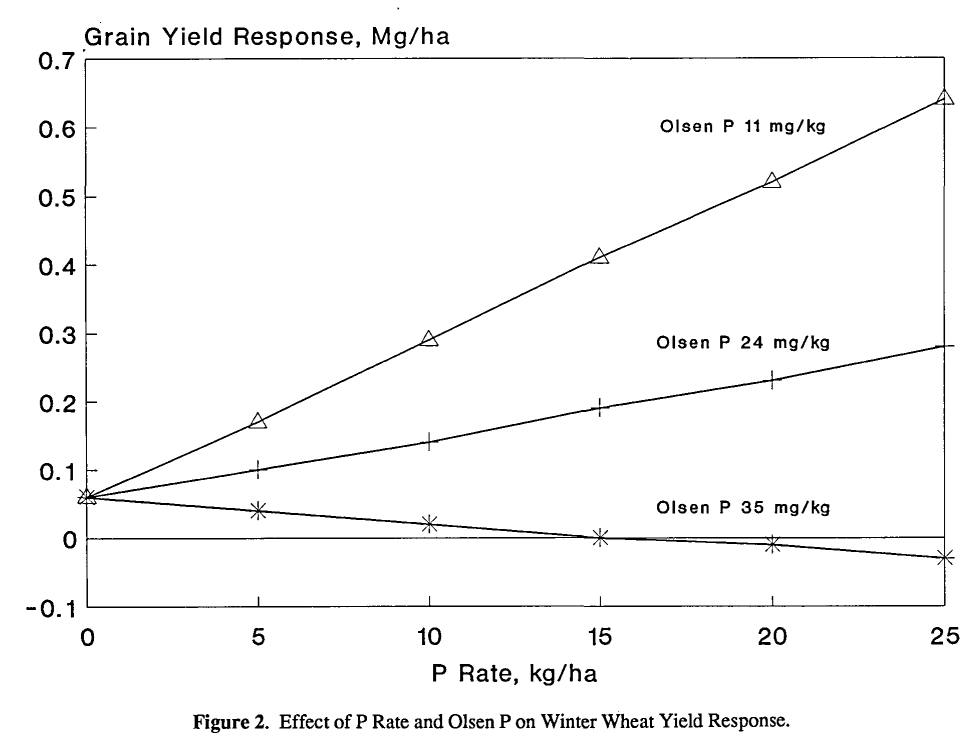
\includegraphics[width=0.65\linewidth]{../images/olsen_p_levels_yield_changes_winter_wheat_US.PNG}
  \end{center}
  \column{.3\linewidth}
  \caption{\newline\tiny Fertilizer response (FR) as function of maize yield in the unfertilized control plots (a, b) or N application rate (c, d) for Sub-Saharan Africa (a, c) and Kenya (b, d). Dashed lines represent no fertilizer response to the fertilizer (FR = 1). The solid lines describe non-linear relationship function as: FR = $\mathrm{32,244 (control~yield)^{-0.7}}$ with significant associations for Kenya and FR = $\mathrm{83 (control~yield)^{-0.5}}$ with significant associations for Sub-Saharan Africa; Source: \cite{ichami2019fertilizer}}
  \label{fig:yield-response-n-sahara}
  
  \end{columns}
\end{figure}
\ecolumns
\end{frame}

\begin{frame}{}
\protect\hypertarget{section-7}{}
\small

\begin{itemize}
\tightlist
\item
  Soil mapping has been widely used to develop statistical models of the
  relationships between environmental variables and soil attributes.
\item
  Obvious applications of soil mapping include:

  \begin{itemize}
  \footnotesize
  \item determining and mapping the spatial distribution of the variability in soil chemical properties of the agricultural lands
  \item develop soil test based fertilizer prescription under Integrated Plant Nutrition System (STCR-IPNS) for various crops and soils
  \item evaluate the extent to which fertilizer needs of crops can be reduced with the conjoint use of organic manures
  \item evaluation of various soil test methods for their suitability under field conditions
  \end{itemize}
\item
  Field level soil sampling and testing services (as campaigns and
  routine tests) in Nepal are offered by

  \begin{itemize}
  \footnotesize
  \item Government organizations (Central Soil Testing Laboratory, Provincial Soil Testing Laboratory, Municipal level soil testing laboratories, National Soil Research Center (NSSRC)-NARC, University Departments (Central Department of Geology))
  \item Non-government Organizations
  \item Private laboratories
  \end{itemize}
\end{itemize}
\end{frame}

\begin{frame}{Digital soil map (of Nepal)}
\protect\hypertarget{digital-soil-map-of-nepal}{}
\begin{figure}
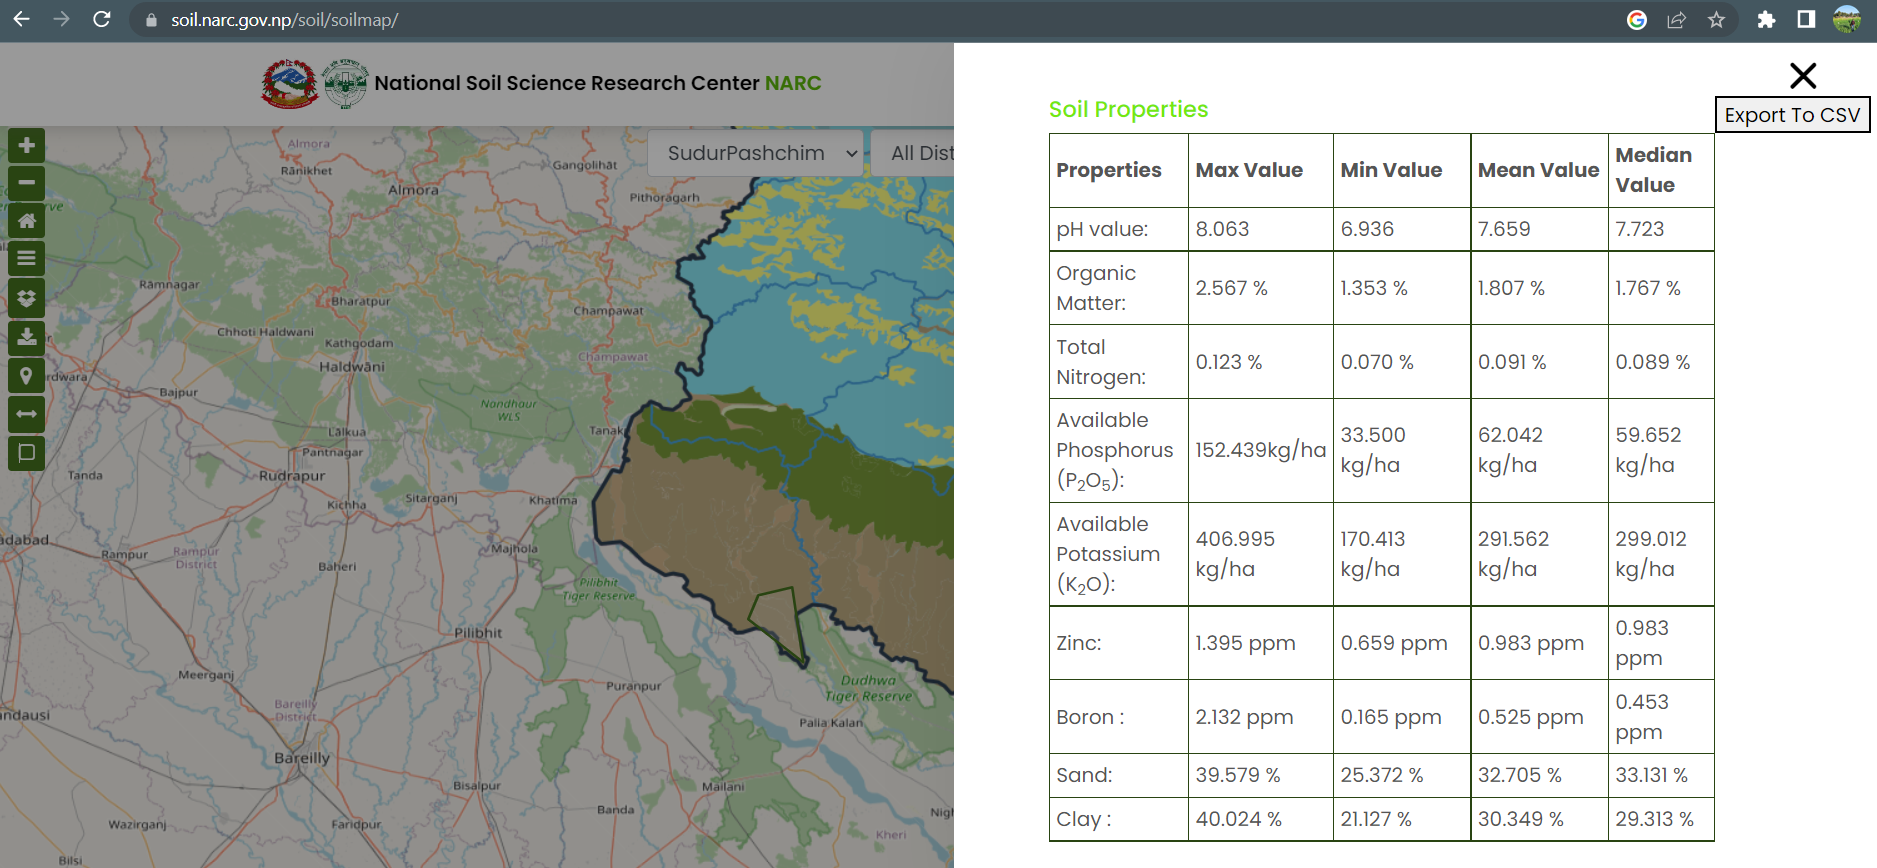
\includegraphics[width=0.8\linewidth]{../images/digital_soil_map_nepal_narc} \caption{Digital soil map of Nepal, showing soil attributes for selected region (South-eastern part of Kailali district). NARC's National Soil Science Research Center (NSSRC) in partnership with USAID's Nepal Seed and Fertilizer (NSAF) project developed the web based application.}\label{fig:digital-soil-map-nepal}
\end{figure}
\end{frame}

\begin{frame}{}
\protect\hypertarget{section-8}{}
\small

\begin{itemize}
\tightlist
\item
  Digital Soil Map (DSM) is a computer-assisted production of digital
  maps of soil properties. This is developed by using mathematical and
  statistical models that combine soil information from laboratory
  analysis with environmental variables (soil forming factors).
\item
  Soil mapping is assisted for realistic appraisal of environmental
  factors (allowing for adjustment) that affect soil properties.

  \begin{itemize}
  \tightlist
  \item
    Covariate layers are generated using satellite images (raster data)
  \item
    Important factors are topographic data, vegetation, precipitation,
    temperature, soil parent material, land cover type, landform
    classes.
  \end{itemize}
\item
  DSM uses advanced computational algorithms that use both soil sample
  data and environmental variables to generate maps. It does not only
  use spatial autocorrelation as the means to interpolate the data, but
  also considers soil forming factors. Also, the process can be
  automated so that newer versions of the map can be developed faster
  once new soil samples are collected. As soil properties are combined
  with environmental variables, a smaller number of soil samples would
  be enough to generate DSM compared to conventional soil map.
\end{itemize}
\end{frame}

\begin{frame}{}
\protect\hypertarget{section-9}{}
\footnotesize

\begin{itemize}
\tightlist
\item
  Recently `Digital Soil Map Management Guidelines, 2078' has been
  implemented.
\item
  Digital soil map for Nepal provides access to location-specific
  information on soil properties for any province, district,
  municipality or a particular area of interest. The interactive map
  provides information that will be useful to make new crop-and
  site-specific fertilizer recommendations for the country.

  \begin{itemize}
  \footnotesize
  \item Soil map: \url{https://soil.narc.gov.np/soil/soilmap/}
  \item Crop map: \url{https://soil.narc.gov.np/crop/cropmap/}
  \end{itemize}
\item
  Spatial resolution of the maps is 250 m.
\item
  Prepared using soil information from 23,273 soil samples collected
  from the National Land Use Project, Central Agricultural Laboratory
  and Nepal Agricultural Research Council. The samples were collected
  from 56 districts covering seven provinces. These soil properties were
  combined with environmental covariates (soil forming factors) derived
  from satellite data and spatial predictions of soil properties were
  generated using advanced machine learning tools and methods.
\item
  Help to increase crop yields and also the nutritional value of these
  crops
\end{itemize}
\end{frame}

\hypertarget{common-issues-of-precision-agriculture-for-nepal}{%
\section{Common issues of precision agriculture for
Nepal}\label{common-issues-of-precision-agriculture-for-nepal}}

\begin{frame}{}
\protect\hypertarget{section-10}{}
\begin{columns}[T, onlytextwidth]
\column{0.5\textwidth}

\begin{itemize}
\item Farmers commonly split large, undulating crop fields, even those at similar elevation range or contour, into a
patchwork of small sub-plots in plane areas of Nepal.
\item Use of hotbeds, coldframes, shade house in horticulture.
\item Drone assisted diagnostics and prescription agriculture (DADAPA)
\item Cloud marketing system (CMS)
\end{itemize}

\column{0.5\textwidth}


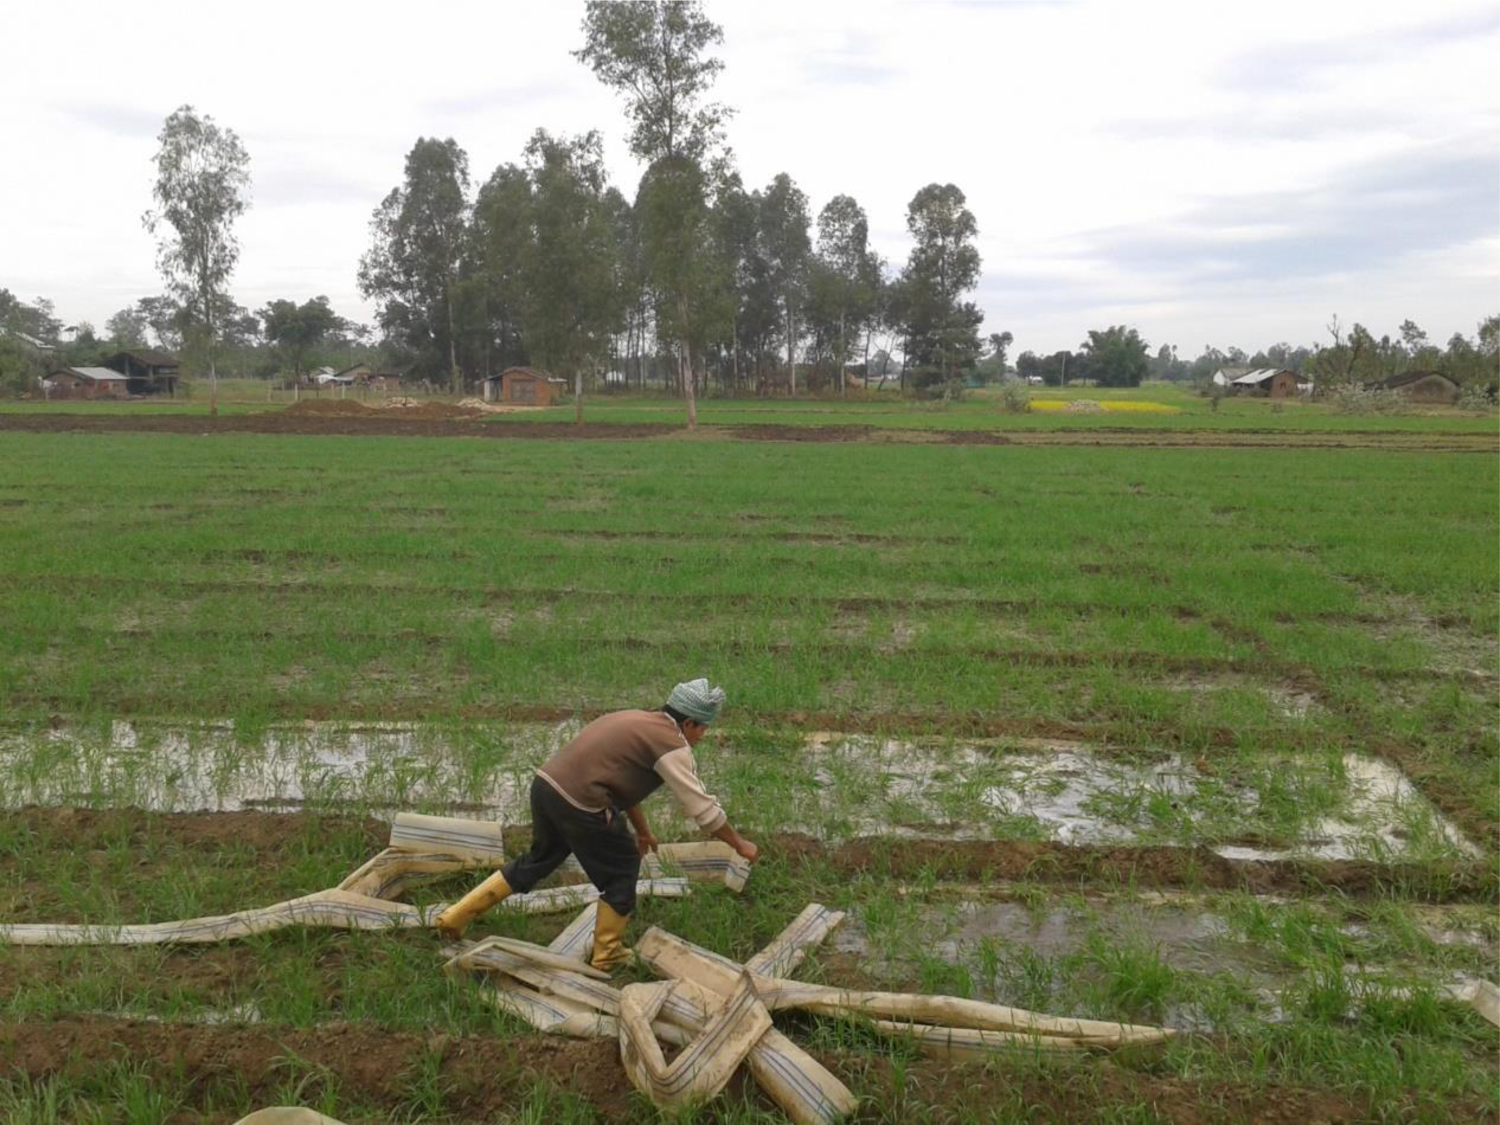
\includegraphics[width=0.9\linewidth]{../images/irrigating_farmer} 

\end{columns}
\end{frame}

\begin{frame}{Issues with precision agriculture in Nepal}
\protect\hypertarget{issues-with-precision-agriculture-in-nepal}{}
\begin{itemize}
\tightlist
\item
  Implementation of PA is fundamentally different for developed and
  developing country.
\item
  Average land holding in Nepal is \textless0.6 ha per household.
\item
  More than 80\% of the farmers are smallholder and are practicing
  subsistence farming.
\item
  Modern form of precision farming hinges on skilled human resources for
  its adoption

  \begin{itemize}
  \tightlist
  \item
    knowledge about IoT and IT technologies
  \item
    use of recent innovations and research
  \end{itemize}
\item
  Lays emphasis on extensive mechanization
\item
  Adds to the cost of smallholder
\item
  Financial support systems are underdeveloped
\item
  Slower adoption rate (social structure); besides being technology
  averse, smallholders may often hinder the progress of expansion of
  technology
\item
  Existing infrastructure bottleneck

  \begin{itemize}
  \tightlist
  \item
    irrigation
  \item
    roadways
  \end{itemize}
\end{itemize}
\end{frame}

\begin{frame}{Possible solutions}
\protect\hypertarget{possible-solutions}{}
\begin{itemize}
\tightlist
\item
  professional human resource development;
\item
  policy initiated and/or supported investments into infrastructure;
\item
  affordable handsets and reduced device costs;
\item
  available and affordable access to Internet for the farmers funded by
  different institutions (public or donor financed);
\item
  solutions between low- and high-level services (e.g.~between SMS and 4
  or 5G networks).
\item
  development and open publication of site specific soil maps, supported
  by public institution.
\end{itemize}
\end{frame}

\hypertarget{bibliography}{%
\section{Bibliography}\label{bibliography}}

\begin{frame}{References}
\protect\hypertarget{references}{}
\end{frame}

          \begin{frame}[allowframebreaks]{}
    \bibliographytrue
    \bibliography{./../bibliographies.bib}
    \end{frame}
  


\end{document}
